\section{Conception}
\subsection{Conception préliminaire}

\subsubsection{Diagrammes de séquence}
Les diagrammes de séquences correspondant aux différentes actions possibles des clients et des administrateurs du site sont présentés ci-dessous.

Voici le diagramme de séquence pour l'inscription sur le site.

\begin{figure}[H]
\begin{centering}
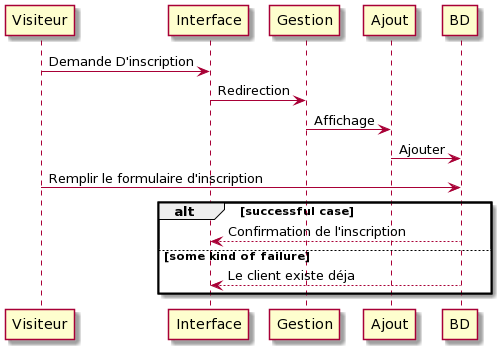
\includegraphics[width=0.95\textwidth,height=0.6\textheight]{Ressources/Inscription.png}
\caption{Diagramme de séquence pour l'action ``inscription''}
\par
\end{centering}
\end{figure}

\clearpage

Voici le diagramme de séquence pour se connecter sur le site.

\begin{figure}[H]
\begin{centering}
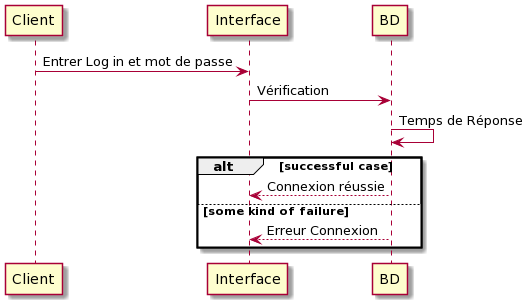
\includegraphics[width=0.95\textwidth,height=0.6\textheight]{Ressources/Login.png}
\caption{Diagramme de séquence pour l'action ``login''}
\par
\end{centering}
\end{figure}

\clearpage

Voici le diagramme de séquence correspondant à l'action de commander qu'un client peut effectuer sur le site.

\begin{figure}[H]
\begin{centering}
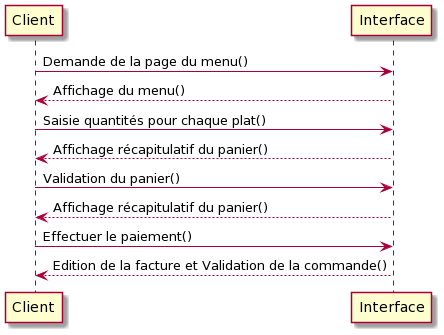
\includegraphics[width=0.95\textwidth,height=0.6\textheight]{Ressources/Commander.png}
\caption{Diagramme de séquence pour l'action ``commander''}
\par
\end{centering}
\end{figure}

\clearpage

\subsubsection{Diagrammes de navigation}
Ci-dessous se trouvent nos diagrammes de navigation qui présentent l'architecture des pages de notre site.

Voici le diagramme de navigation pour les administrateurs.

\begin{figure}[H]
\begin{centering}
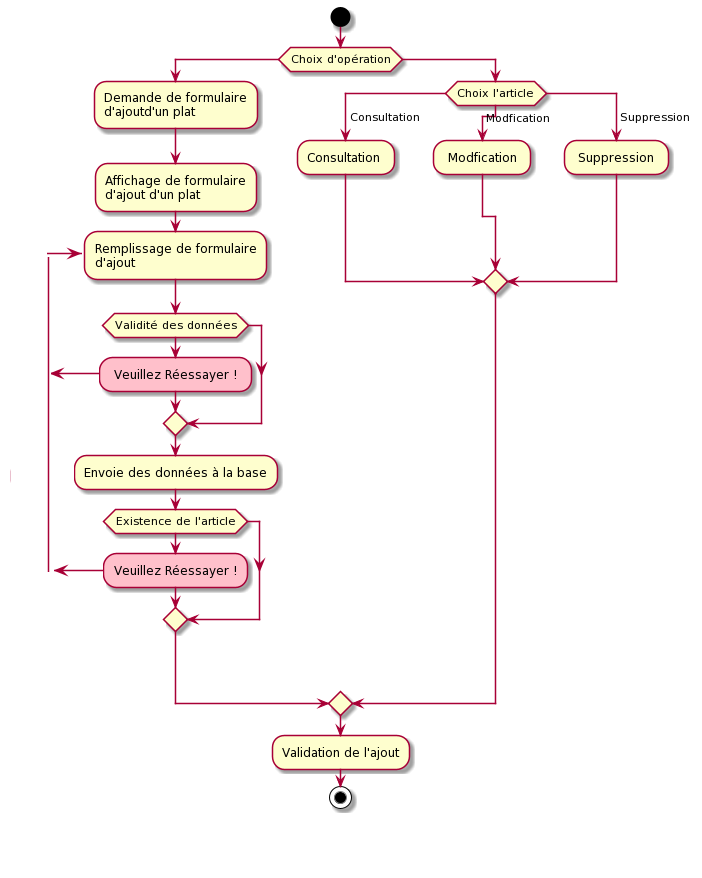
\includegraphics[width=0.7\textwidth,height=0.8\textheight]{Ressources/Administrateur_navigation.png}
\caption{Diagramme de navigation pour les administrateurs}
\par
\end{centering}
\end{figure}

\clearpage

Voici le diagramme de navigation pour l'inscription.

\begin{figure}[H]
\begin{centering}
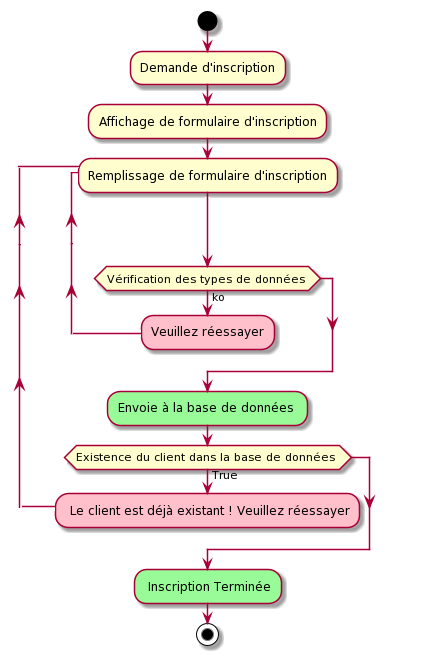
\includegraphics[width=0.7\textwidth,height=0.85\textheight]{Ressources/Inscription_navigation.png}
\caption{Diagramme de navigation pour l'inscription}
\par
\end{centering}
\end{figure}

\clearpage

Voici le diagramme de navigation pour le login.

\begin{figure}[H]
\begin{centering}
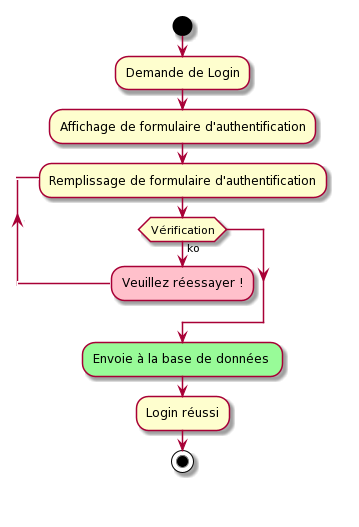
\includegraphics[width=0.7\textwidth,height=0.85\textheight]{Ressources/Login_navigation.png}
\caption{Diagramme de navigation pour le login}
\par
\end{centering}
\end{figure}

\clearpage

\subsubsection{Diagramme de relation entre les pages}
Voici le diagramme de relation qui montre les relations existant entre les différentes pages du site web.

\begin{figure}[H]
\begin{centering}
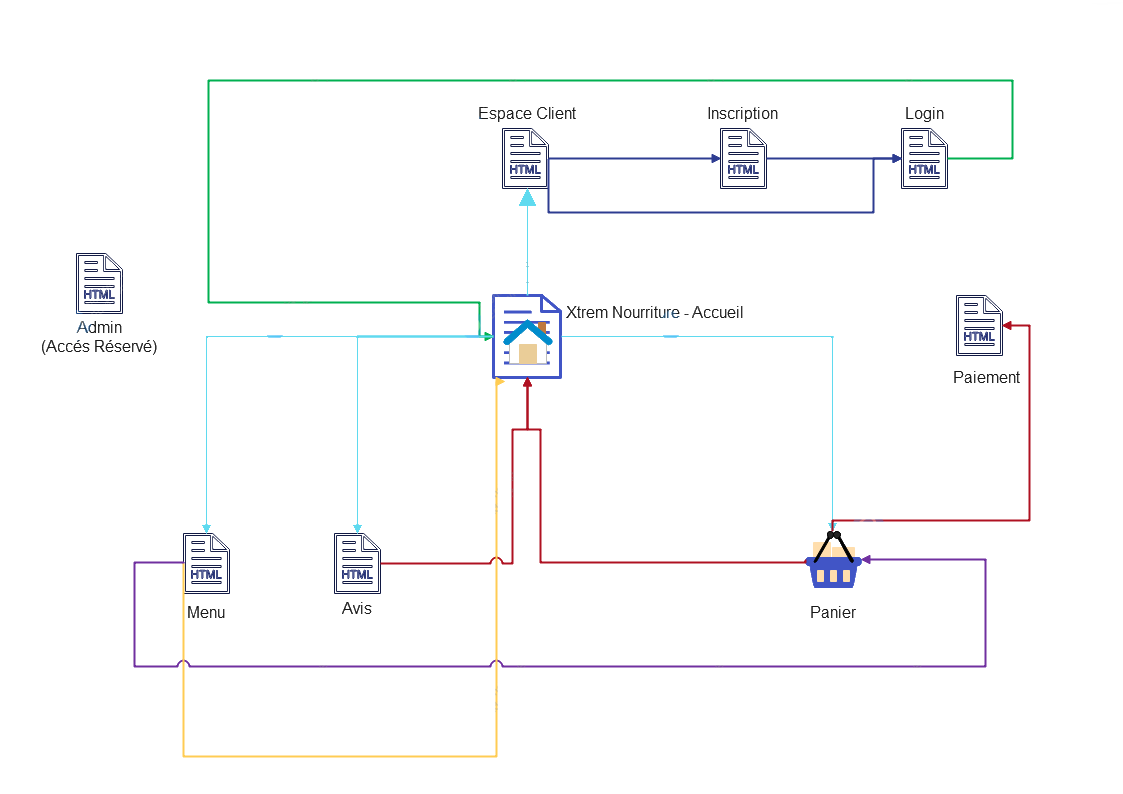
\includegraphics[width=0.9\textwidth,height=0.6\textheight]{Ressources/LaCarteDesSite.png}
\caption{Diagramme représentant la Carte du site}
\par
\end{centering}
\end{figure}

\clearpage

\subsection{Conception détaillée}
\subsubsection{Diagrammes de classe}
On présente ci-dessous les diagrammes de classe correspondant à notre mise en oeuvre du site.

Voici le diagramme de la classe DAO qui constitue l'interface avec la base de données.
\begin{figure}[H]
\begin{centering}
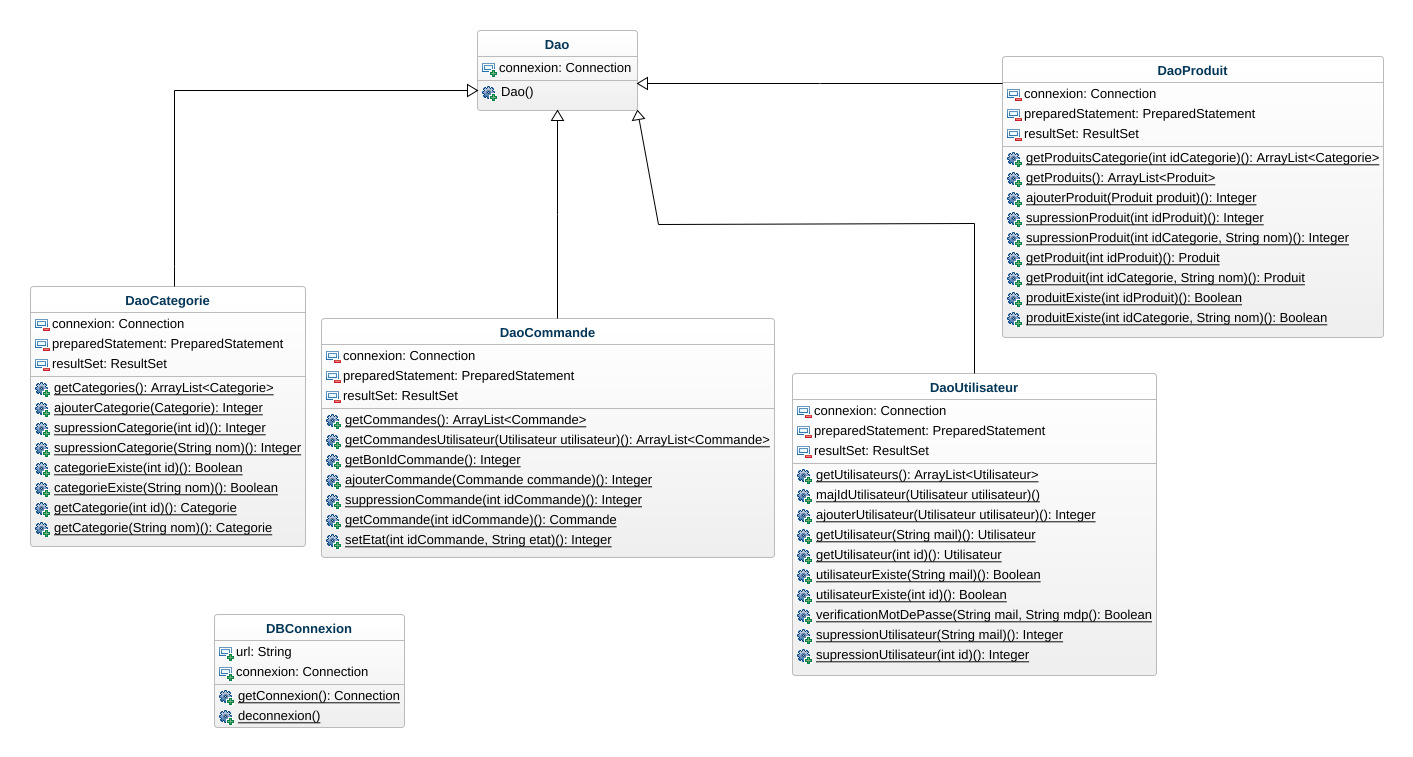
\includegraphics[width=0.95\textwidth,height=0.5\textheight]{Ressources/class-diagram-dao.png}
\caption{Diagramme de classe pour le DAO}
\par
\end{centering}
\end{figure}

\clearpage

Voici le diagramme de classe explicitant nos Javabean.
\begin{figure}[H]
\begin{centering}
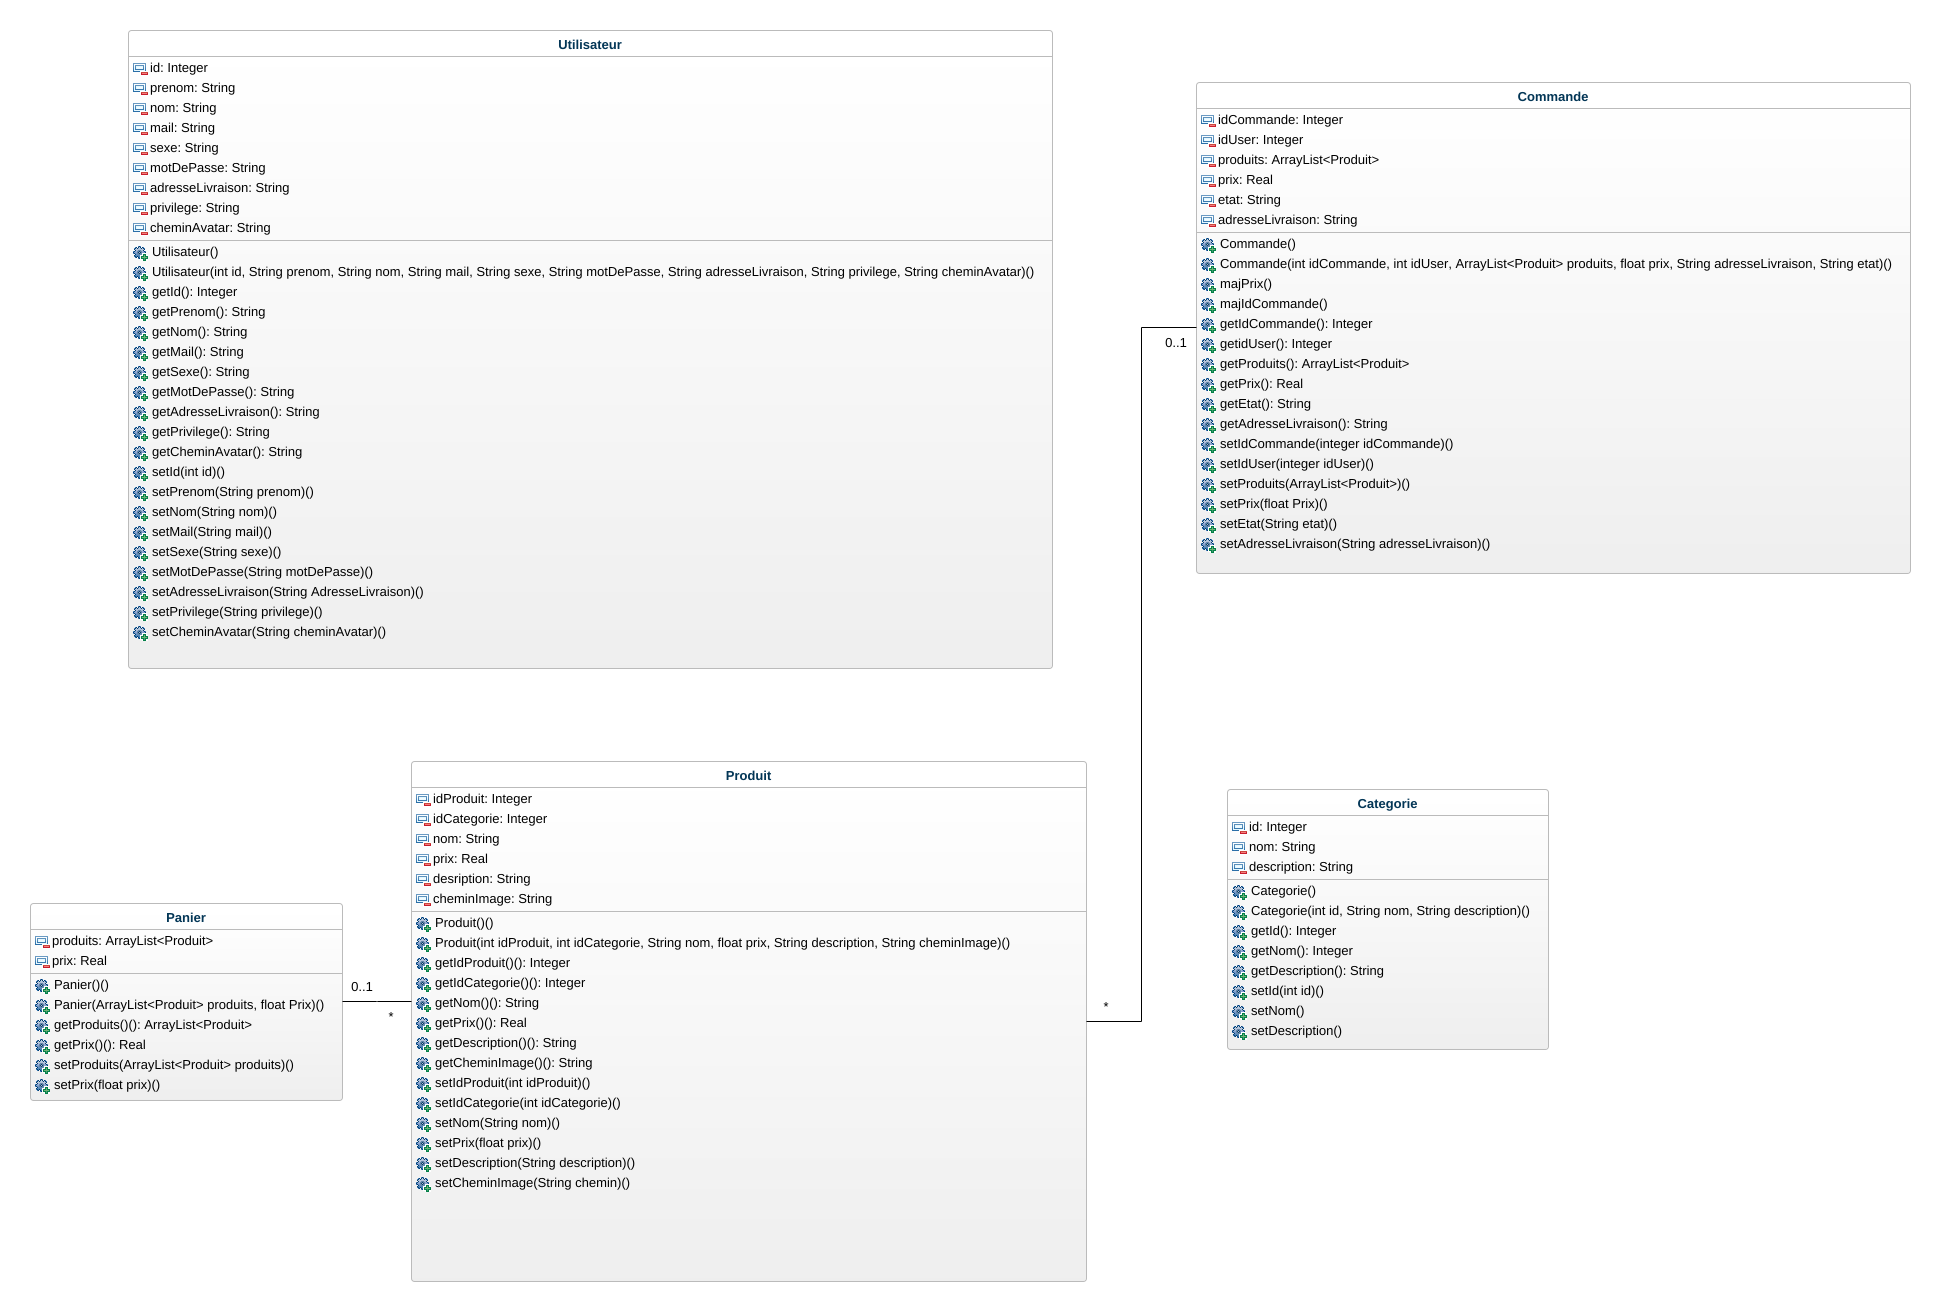
\includegraphics[width=0.9\textwidth,height=0.7\textheight]{Ressources/class-diagram-bean.png}
\caption{Diagramme de classe pour les Javabean}
\par
\end{centering}
\end{figure}

\clearpage

\subsubsection{Représentation logique de la base de données}
Enfin, nous avons représenté ci-dessous une représentation logique de notre base de données.
\begin{figure}[H]
\begin{centering}
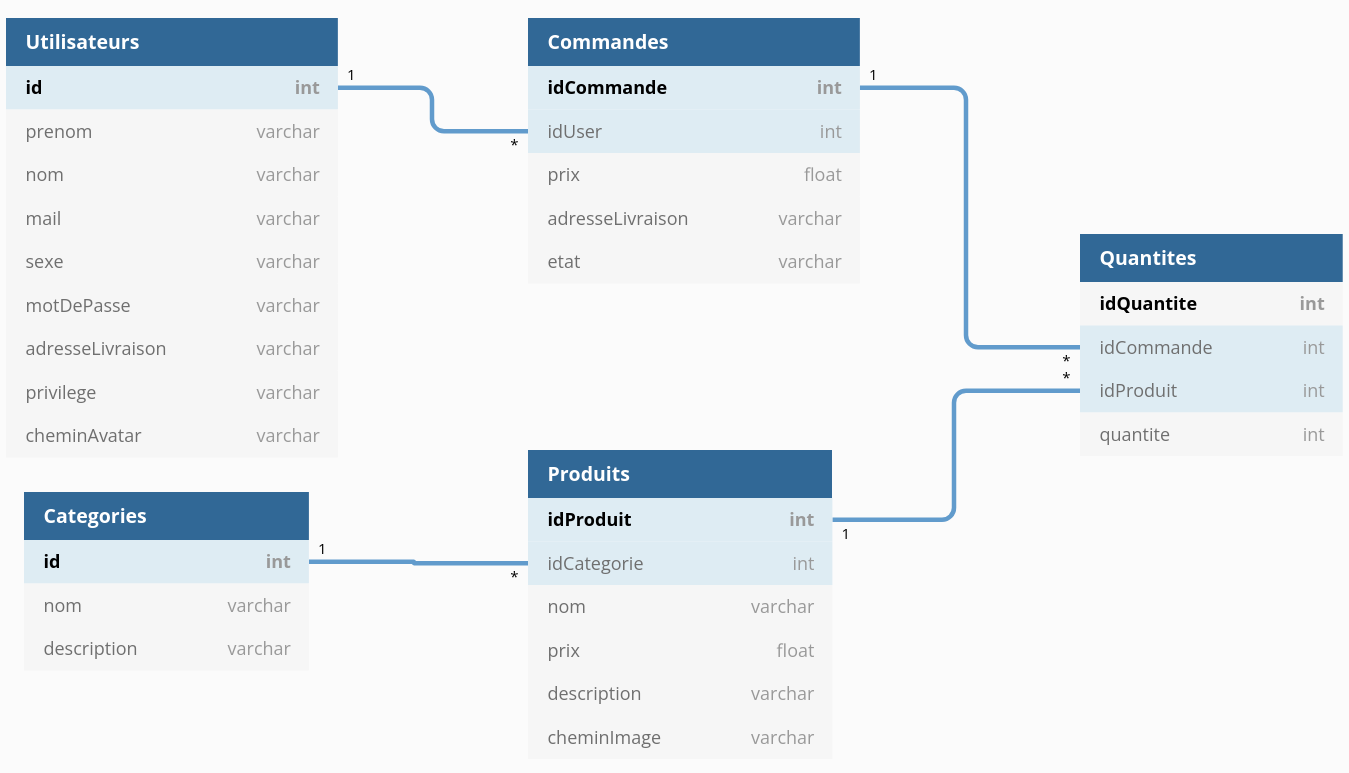
\includegraphics[width=0.95\textwidth,height=0.5\textheight]{Ressources/db-diagram-2.png}
\caption{Représentation logique de la base de données}
\par
\end{centering}
\end{figure}
